\chapter{About expression visualisation, correlation and clustering}
%\chapter{More quality checks and data preparation}
\label{ch:expression}

\begin{comment}
\setlength{\epigraphwidth}{\textwidth}%0.6
\setlength{\epigraphrule}{0pt}%0.1
\epigraphhead[70]{%
\epigraph{[..] 80\% of the data analysis task is spent on cleaning and
understanding the data.}{\cite{Dasu2003-bg}}%
}
\end{comment}

As a first step towards the meta-analyses\footnote{Across transcriptomes,
across proteomes and then across transcriptomes/proteomes.},
I have opted for a semi-empirical approach to determine
a consensus set of methods and parameters on each individual study
before applying them across all the datasets in the further chapters.
This strategy has also allowed me
to estimate the data overall quality per dataset and to tidy them appropriately.

I report quality checks in \Cref{ch:datasets}
that happened before the processing of the data.
Those quality assessments are rather technical\footnote{Is it true signal
or noise?
Are all the nucleotides called?
Is it a true identification or a \gls{FDR}?~\ldots}.
In the present chapter, I describe post-processing quality (or sanity) checks
that examine higher (and fuzzier) aspects, \eg:
%\KOMAoptions{parskip=never}
\begin{itemize}[topsep=0pt,nosep]
    \item Any outlier in the data?
    \item Systematic and unsystematic \emph{batch effects} within each study
    \item Adequacy of data, concepts and statistical models
\end{itemize}
%\KOMAoptions{parskip=half*}
Even if every aspect may not be addressed or corrected the
final results and their interpretations are more solid.

\section{Visualisation of expression data}

Visualising the data first is a very effective method towards adequate analyses
and more pertinent results by uncovering
the detection of underlying structures and possible unwanted artefacts.

\subsection{Distribution plots}\label{subsec:distribPlot}

In the literature, the distribution of expression values are frequently
visualised on a log-scale ($\log_{2}(x)$).
\Cref{fig:distribPlot} and~\Cref{fig:distribPlot_noLog2} illustrate how
this scaling improves the readability of the figure.
Furthermore, the log-scale allows to transform count data to continuous
while smoothing the global distribution shape towards a normal distribution.
Thus, another advantage of this transformation is to conform the data
to many ready available statistical models.

\NB\ Whenever removing the null values is harmful statistically
or for correct interpretation,
I have added a common \emph{pseudocount} (equals to $1$)
to overcome the lack of definition of $\log_{2}(0)$.

\Cref{fig:distribPlot} shows that all \gls{RNA} samples present a similar
profile on this $\log_{2}(x+1)$ scale:
a pic near $0$ for the lowly (and not expressed genes) and a long-trailing tail.
The bulk of the expressed genes on this scale is below $6$ (\ie\ below 63 \FPKM).
Besides, in \Cref{fig:densityUhlen_log2}, we can observe that the general expression
of the pancreas is shifted towards the left in comparison of the other tissue.
This is probably an artefact as this shift is absent in the other pancreas
tissue samples of other transcriptomic datasets.

Aside from the \pandey\ data (\cref{fig:densityPandey_log2}),
the expression of the proteins is more heterogeneous
(in particular \cutler\ data, see \cref{fig:densityCutler_log2}).
This is concordant to the more disparate and various techniques involved in
the proteomic sample preparation (see \cref{subsec:ProtSampPrep}).


\begin{figure}
    \centering
    \begin{subfigure}[b]{0.35\textwidth}
        \centering \includegraphics[width=\textwidth]{expressed/density_Log2/castle.pdf}
        \caption{Castle}\label{fig:densityCastle_log2}
    \end{subfigure}%
~%
    \begin{subfigure}[b]{0.35\textwidth}
        \centering \includegraphics[width=\textwidth]{expressed/density_Log2/vt.pdf}
        \caption{Brawand}\label{fig:densityBrawand_log2}
    \end{subfigure}

    \begin{subfigure}[b]{0.35\textwidth}
        \centering \includegraphics[width=\textwidth]{expressed/density_Log2/ibm.pdf}
        \caption{Illumina Body Map}\label{fig:densityIBM_log2}
    \end{subfigure}%
~%
    \begin{subfigure}[b]{0.35\textwidth}
        \centering \includegraphics[width=\textwidth]{expressed/density_Log2/uhlen.pdf}
        \caption{Uhlen}\label{fig:densityUhlen_log2}
    \end{subfigure}

    \begin{subfigure}[b]{0.35\textwidth}
        \centering \includegraphics[width=\textwidth]{expressed/density_Log2/gtex.pdf}
        \caption{Gtex}\label{fig:densityGtex_log2}
    \end{subfigure}%
~%
    \begin{subfigure}[b]{0.35\textwidth}
        \centering \includegraphics[width=\textwidth]{expressed/density_Log2/cutler.pdf}
        \caption{Cutler}\label{fig:densityCutler_log2}
    \end{subfigure}

    \begin{subfigure}[b]{0.35\textwidth}
        \centering \includegraphics[width=\textwidth]{expressed/density_Log2/kuster.pdf}
        \caption{Kuster}\label{fig:densityKuster_log2}
    \end{subfigure}%
~%
    \begin{subfigure}[b]{0.35\textwidth}
        \centering \includegraphics[width=\textwidth]{expressed/density_Log2/pandey.pdf}
        \caption{Pandey}\label{fig:densityPandey_log2}
    \end{subfigure}
    \caption{Profile of expression across the transcriptome (protein coding
    genes only) and proteome datasets}\label{fig:distribPlot}
\end{figure}

\subsection{Scatter plots}

\cite{anscombe} created four datasets (see \Cref{fig:Anscombe})
which share similar descriptive statistics to show the importance
of data visualisation even through a simple scatter plot.
He demonstrated that checking the datasets graphically with scatter plots
allows to quickly detect outliers and roughly estimate
the relationship between two variables.
Even a non-linear but strong relationship is promptly highlighted
(\eg\ top right corner of~\cref{fig:Anscombe}).

\begin{figure}
    \centering
    \begin{subfigure}[b]{0.45\textwidth}
        \centering \includegraphics[width=\textwidth]{expressed/RepTechscat.pdf}
        \caption{Technical replicates (Heart)}\label{fig:scatTechRep}
    \end{subfigure}~%
    \begin{subfigure}[b]{0.45\textwidth}
    \centering \includegraphics[width=\textwidth]{expressed/RepBiolscat.pdf}
        \caption{Biological replicates (Kidney)}\label{fig:scatBiolRep}
    \end{subfigure}
    \caption{Examples of scatter plot for replicates from \uhlen\
    (transcriptome)}\label{fig:scatEg}
\end{figure}

\Cref{fig:scatTechRep} illustrates how very lowly expressed \gls{RNA}
diverge even in technical replicates.
Biological replicates, within a same dataset,
may present very close profiles though with a greater spread
as showed in \Cref{fig:scatBiolRep}.


\section{Main statistical approaches}

\subsection{Correlation}
%Cum hoc ergo propter hoc

Correlation coefficients are a measure of the statistic dependence between two
continuous variables\footnote{In the context of this study: either expression
levels of a given gene across samples/tissues or expression levels of all genes
\emph{between} two samples or tissues} (\eg\
$X$ and $Y$) and always ranges within $[-1,1]$ (see also \cref{sec:CorrMore}).

The correlation coefficient is computed by pairwise comparing observations
between the two variable. Most implementation methods
will manage an unbalanced number of observations by excluding the incomplete pairs.
To ease the interpretation I preferred to filter the data \latin{a priori}
myself; I only kept expression values \emph{effectively observed}
in all the datasets (see~\cref{sec:ExpressedOrNot}).

Among the several methods available to compute the correlation coefficient, I
tried both the Spearman and the Pearson correlations
(see respectively \cref{subsec:SpearmanCor} and \cref{subsec:PearsonCor}).

\subsection{Clustering analysis}

As we know the tissue type for each sample of each dataset,
we may debate that supervised analyses can be more informative.
However, they would involve proper corrections for batch effects and
other technical biases for each dataset.
This is challenging as that often requires more knowledge than the available one
through the repositories.
In \Cref{ch:datasets}, we have seen it is also unwise to rely solely on the
normalised data provided by the original authors\footnote{Eventual bias
corrections in \Rnaseq\ vary according to planed downstream analyses and
proteomic data is hard to handle and two processing pipelines may rather give
quite different results (see~\Cref{ch:proteomics}).}.

To assess the consistency of the quantification across the different datasets,
in particular for \Rnaseq,
I picked a widely used and unsupervised method for gene expression studies:
a clustering analysis.
This method uncovers possible hidden
structures within the data, therefore,
it is well designed for exploratory studies.
I can thus confirm if samples are more alike either due to their
biological or their study origins.

In general, we expect biology to be a better predictor when we only consider
data from either transcriptome or proteome. Even more so, if the
identification technology and the quantification workflows are
consistent. Yet, a technical predictor can not be excluded straightforwardly.
Indeed, most transcripts (in particular \mRNAs) are expressed in many tissues
and two random tissues share about 60 to 90\% of their pool of
\mRNAs~\mycite{ramskoldan:2009,UhlenGastro}.
Coincidentally, on the proteome side,~\cite{PandeyData}
estimate that 75\% of the mass of a cell is due to ubiquitous proteins and
\cite{KusterData} estimate that about 10,000
to 12,000 proteins are ubiquitously detected, which represent about 60 to 75\%
of the proteins that they identified per tissue. Thus, if the variation of
expression are too subtle from one tissue to another, a strong sample collection
or data processing bias may hide any relevant biological signal.

There are many available approaches and algorithms for clustering analysis.
I~chose a (bottom-up) \emph{hierarchical} clustering (a.k.a.\
\emph{connectivity-based} clustering).

This sort of clustering is broadly used in gene expression studies as it is
embryologically\footnote{Or evolutionary, when different species are compared}
pertinent\footnote{The whole organism develops from
an original single cell.}. The data is portioned in an extensive hierarchy:
each cluster merges with another at a certain distance.
In practice, each sample starts in its own cluster and then
by iteration, each cluster is merged with its nearest one.
The method has two parameters: the distance and the linkage method.
Debate is still going on how to pick these parameters (for more details
see~\mycite{Jaskowiak2014}).

The distance measures the dissimilarity between two samples and one common
approach is to calculate the subtraction result of
the correlation coefficient from $1$ (hence, a greater similarity between the two
samples means a smaller distance). As previously, I have also used both Spearman
and Pearson correlation methods.

The linkage parameter specifies which part of each cluster is used as reference
for computing the distance between the clusters. There are many methods and after
trying several, I have arbitrary selected the one that divides the most accurately
the samples by their tissue source across the different datasets.
In fact, I noticed that the Ward's method~\mycite{Ward1963}
was the best for this task and was outperforming the complete-linkage method.
Indeed, this later method was used in~\mycite{Uhlen2014}
(first release of the \uhlen\ dataset) where
the original authors have to discard a few samples as they were clustering
incoherently in regards of their biological nature.
However, the Ward's method allows to conserve all the samples for the analysis
as long as another bias source is corrected (see \cref{subsec:mito}).


\section{Reducing obvious bias sources}

Many non-trivial methods correct for the skewness presents in
\Rnaseq\ and \ms-based proteome global expression distributions
and for other possible bias sources.
However, it may be complex to assess the biological relevance of those corrections.
Hence, while it may be better to correct for every bias in principle,
in the context of this thesis, this is a smaller concern as I am interested into
consistent traits across the datasets that may be consolidated into a reference.
Nonetheless, prior to the analysis and while its early stages,
I found a few easily avertible biases that I describe hereinafter.

\subsection{Protein coding genes}
I have focused my analyses on the \mRNAs\ (\ie\ \glspl{RNA} that have a
biotype described as \emph{protein coding} in \ens{76}).

In addition of the obvious reason to match with the proteomic data,
most of the transcriptomic data is the produce of poly-A selected protocols
(see \cref{msec:polyA}).
Thus, aside of the \mRNAs, all the other \glspl{RNA} are off-target
and, for many of them,
their expression levels estimations may be highly imprecise.

\subsection{Mitochondria issue}\label{subsec:mito}

Gene expression levels of mitochondria can report very useful information,
\eg\ the stress level of a cell in a single cell experiment~\mycite{Ilicic2016}.
However, it is unwise to keep them for a bulk analysis, particularly when
comparing different biological sources.
Indeed, it is very hard to properly normalise their expression.
It involves knowing the amount of mitochondria in the studied samples.
I have decided to remove them from the analysis as they skew anything relying
on correlation.
In fact, there are always mitochondrial genes among the highest expressed genes
and they usually dominate manifolds the expression of the other genes.

Removing the 37 mitochondrial genes from the bulk of expressed genes
(above 10,000 protein coding genes) produces more defined clusters as showed on
\Cref{fig:MitoNomito}.

\begin{figure}
    \centering
    \begin{subfigure}[b]{0.75\textwidth}
        \centering
        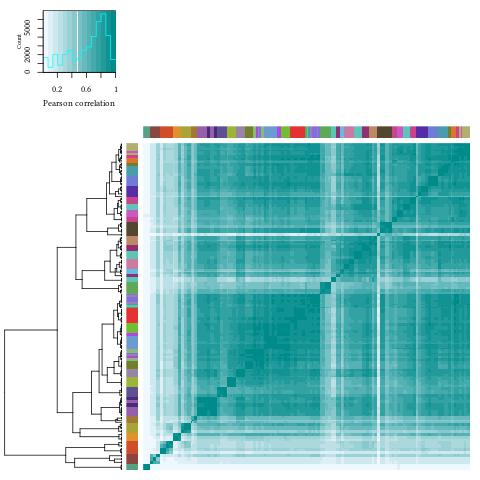
\includegraphics[width=\textwidth]{expressed/Uhlen_noLog_mito_htseq.pdf}
        \caption{With the 37 mitochondrial genes}\label{fig:withMito}
    \end{subfigure}

    \begin{subfigure}[b]{0.75\textwidth}
        \centering
        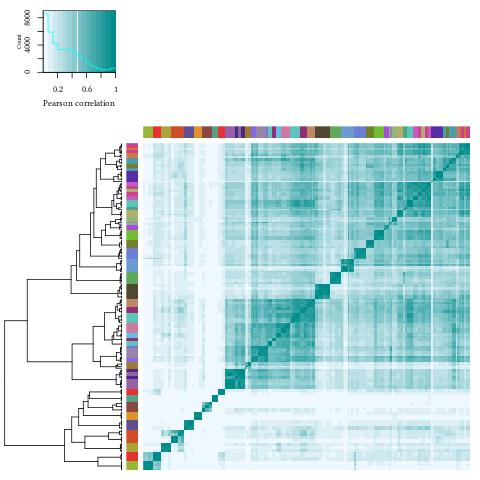
\includegraphics[width=\textwidth]{%
            expressed/Uhlen_noLog_NoMito_htseqPearson.pdf}
        \caption{Without the mitochondrial genes}\label{fig:NoMito}
    \end{subfigure}
    \caption{Clustering of the biological samples of \uhlen\
    dataset based on the Pearson correlation}\label{fig:MitoNomito}
\end{figure}


\subsection{Expressed or not expressed}
\label{sec:ExpressedOrNot}

While it can seem as a trivial concept and might be overlook, whether a specific
molecule is expressed --- or not --- in a given condition, can actually have
an extensive impact on the results of the analyses, particularly when integrating
proteome and transcriptome together.

For example, the Pearson correlation coefficient is very
sensitive to outliers and null values. If for both samples, a vast number of
null values are recorded, this will lead to a greater similarity.
Hence, it is important that the data used for the analysis is meaningful in
its whole, \ie\ a null value has still to be an observation and translates
a lack of expression (and not a lack of observation).

\begin{figure}[!htbp]
    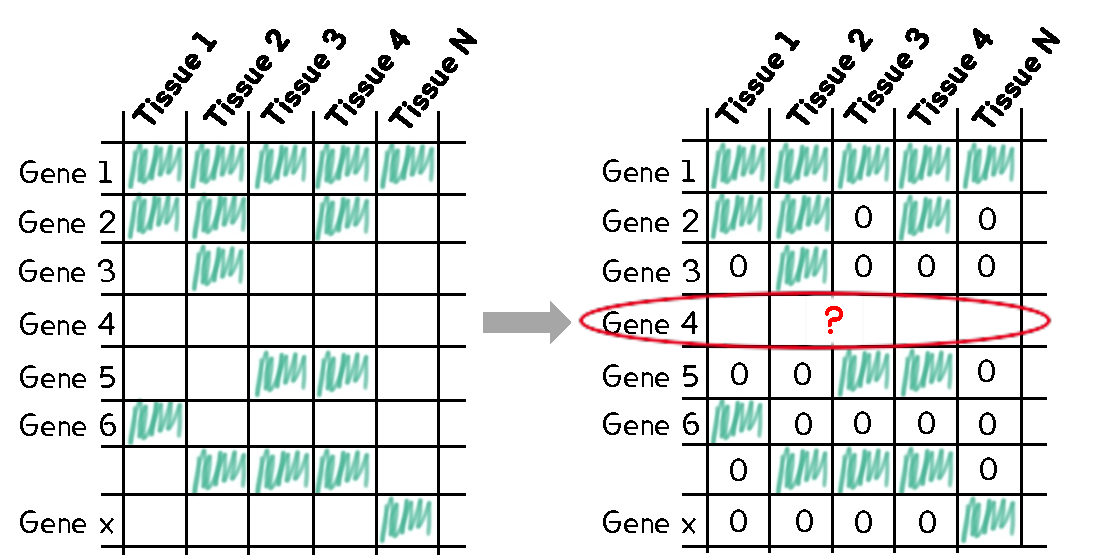
\includegraphics[scale=0.7]{expressed/expressedNotExp.pdf}\centering
      \caption[Expressed or not: several cases illustrated]
      {\label{fig:DefineExpression}\textbf{Expressed or not: several cases
      illustrated.}\smallbreak{} Genes as \emph{gene 1} are unequivocal: they have been
      detected in all the different tissues. Genes that have been quantified in
      \emph{some} of the conditions are, in principle, detectable with the
      protocol of sampling and quantification used for the assay.
      For these genes, when no signal is collected, I assume this is a true $0$.
      The genes without any quantification
      in any tissue, \eg\ gene 4, are discarded from the remaining analysis as
      I can't state
      either there are truly absent from the biological sample or it has to due
      to the protocol at use; they are \emph{undefined}. The same approach is used
      for the transcriptome and the proteome.}
\end{figure}

\subsubsection{The undefined}%\KOMAoptions{parskip=false}
\label{subsec:ExpressedOrNot-undefined}
If a protein or transcript is never found in any of the samples of a dataset,
then I considered that we can not determine if the protein or transcript was
either truly not expressed or, for any reason, was not capture while the library
preparation or the identification/quantification steps. Hence, those are
excluded from the analyses as I can not resolve precisely if this is a
technical artefact or a biological truth. This case is illustrate by the row
circled in red in~\cref{fig:DefineExpression}.

\subsubsection{Expression in a dataset}
\label{subsec:ExpressedOrNot--expDataset}
By contrast, if a protein or a transcript is expressed in some samples of the
dataset, then, whenever no expression was recorded in the other
samples, I consider that the expression of the considered macromolecule is truly
null for those samples.

\subsubsection{Expression within a sample}
Due to the technical (and biological) differences between proteomics and
transcriptomics, I use different thresholds to define the expression of a protein
or a transcript.

\minisec{Expressed protein}
On the proteomic side, I consider that a protein is expressed if it has been
identified and quantified. In other words, if the expression value of a protein
is greater than zero in a sample, I consider it as expressed.

\minisec{Expressed transcript}\KOMAoptions{parskip=half*}\label{subsubsec:exprTrans}
It is a bit more complex on the transcriptomic side as we have to account for
technical noise, but we can also expect \enquote{translational noise}~\mycite{rnaseq-2009},
\mycite{lowNoiseLimit}.
While we can empirically evaluate it for each \Rnaseq\
dataset~\mycite{ramskoldan:2009},
there is a widespread threshold used in the literature:
1 \gls{FPKM} (or \gls{RPKM}).
In fact,~\citet{Hebenstreit:2011} showed in their study
\paper{\citetitle{Hebenstreit:2011}},
that to be detected and quantified as a protein,
a \mRNA\ should at least present an expression equals to 1 \gls{RPKM}.

Hence, I have used this threshold to run (at least once) all the analyses.
As an important part of my thesis focuses on
the comparison of proteomic and transcriptomic data (see \Cref{ch:Integration}),
I have run all the analyses at least with this threshold of $1$ \gls{FPKM}.

It may worth mentioning that I have also redone parts of the analyses without
any threshold (\ie\ I use then the same definition for the \mRNAs\ than for the
proteins) or with a threshold of $5$ \glspl{FPKM}\footnote{While this threshold
may be found in the literature, it remains rather arbitrary.}.

\subsubsection{Limitation of the study}
While I may have compared the list of
undefined, expressed and unexpressed molecules
the bulk of the analyses has been done on the common expressed genes across
the datasets.

In other words, if a \mRNA\ --- or protein --- is not expressed in at least
one sample in \emph{every and each} of the datasets used for the analyses,
I then exclude it.

\subsection{Averaging tissue expression}

Finally, to avoid unnecessary skewness in the meta-analysis due to
the biological replicates unbalance across the datasets (see \cref{sec:expDesign}),
I computed a \emph{\enquote{virtual} reference} for each tissue
for the datasets that present more than one biological sample per tissue,
\ie\ \vt, \uhlen\ and \gtex\ datasets.
Indeed, \castle, \cutler, \kuster\ and \pandey\ datasets present by design only
one measure of expression per gene per tissue.

Thus, for each tissue of \vt, \uhlen\ and \gtex\ datasets, I compute gene
expression levels by taking the median value of each gene across all the
biological replicates of that tissue.

\textbf{Notes:}
\KOMAoptions{parskip=never}
\begin{itemize}[topsep=0pt,nosep]
        \item For \ibm\ dataset, I discard the single-end sequenced samples.
        \item The \uhlen\ dataset has required an extra \emph{prior} step to
            the averaging of the biological replicates
            for some of the tissues as they present technical replicates.
            For these, I have first averaged the gene expression levels
            for each subject-tissue pairs before computing
            the gene expression level medians of each tissue.
        \item On the other hand, the \gtex\ dataset has required another
            \emph{post} step after the averaging of the biological replicates.
            Indeed, in \gtex, the samples are described based on their
            body site sources while the other datasets describe their samples
            only based on their tissue origin.
            Thus, while there is only \tissue{Heart} samples in \castle, \vt,
            \ibm, \uhlen, \cutler, \kuster\ and \pandey,
            \gtex\ has samples from the \tissue{left ventricle of the Heart}
            and from the \tissue{Atrial appendage of the Heart}.
            For this case and other similar ones,
            I have average the virtual reference of the body sites in \gtex\
            that I have appraised as relevant for comparison with tissues found
            in the other datasets.
%see more for esophagus in next chapter.
\end{itemize}
\KOMAoptions{parskip=half*}

\section{Discussion}

In this chapter, I quickly review many fine points that
may be (and often are) overlooked.
While it may be perceived as nitpicking,
these details have critical impact on the results of the analyses
I perform and more gravely on their interpretations\footnote{%
For more, see~\paper{\citetitle{Kratz2014}}~\mycite{Kratz2014}
and the included references.}.

Aside the datasets selection criteria,
this phase is by far the most subjective one of the whole thesis.
Hence, to avoid excessive \emph{data massaging\footnote{I.e.\ data cleaning.}}
and possible cognitive biases,
I have formulated the aforementioned filtering rules
that are important but simple.

Overall, I am quite conservative and I have preferred to keep more data
without any strong rationale to discard them.
Therefore, there are sharper filters and samples exclusion options that
may easily improve the results I present in this thesis.

For example, in my many exchanges with the community,
I was repetitively asked about the inclusion of all the \gtex\ dataset samples
related to \tissue{Oesophagus} for the averaging step.
Indeed, while two of the three body sites present great similarities
to \tissue{Oesophagus} samples of the \uhlen\ dataset,
the last body site expression is very dissimilar.
Thus, excluding this body site will significantly improve
the overall correlation of \gtex\ and \uhlen\ \tissue{Oesophagus}.


